% begin module natural-logarithm-def
\begin{frame}
\frametitle{Natural Logarithms}
\begin{definition}[$\ln x$]
The logarithm with base $e$ is called the natural logarithm, and has a special notation:
\[
\log_e x = \ln x .
\]
\end{definition}
\begin{columns}[c]
\column{.5\textwidth}
\psset{xunit=0.6cm, yunit=0.6cm}
\begin{pspicture}(-5, -5)(5,5) 
\psframe*[linecolor=white](-5,-5)(5,5) 
\psaxes[ticks=none, labels=none]{<->}(0,0)(-4.2,-4.2)(4.2, 4.2)
\psline(-0.1, 1)(0.1,1)
\rput[r](-0.2, 1){\footnotesize$1$}
\psline(1, -0.1)(1,0.1)
\rput[t](1, -0.2){\footnotesize$1$}
\rput[l](1.3, 3.2){\footnotesize$y=e^x$}
%Function formula: 2^{x} 
\psplot[linecolor=red, plotpoints=1000]{-4}{1.386294361}{2.718281828 x exp }
\psplot[linecolor=red, plotpoints=1000]{0.018315639}{4}{x ln}
\psline[linestyle=dashed, linecolor=blue](-4, -4)(4,4) 
\rput[tl](2, 0.7){\footnotesize$y=\ln x$}
\rput[tl](-2, -2.3){\footnotesize$y=x$}
\end{pspicture} 
%\ 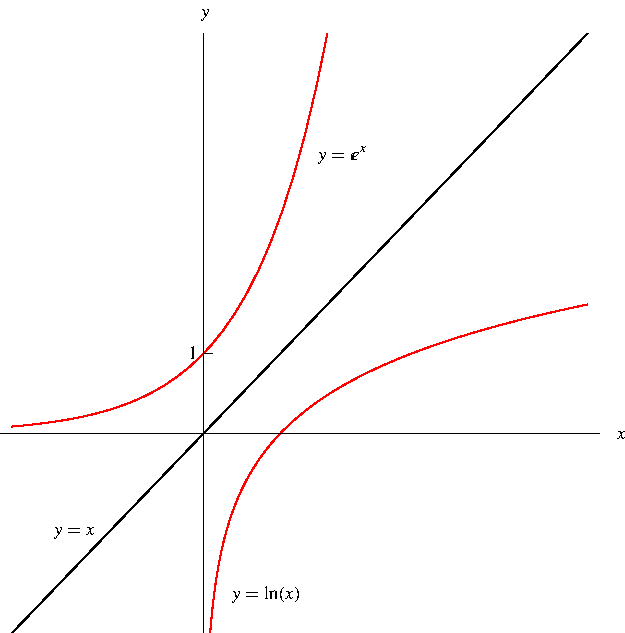
\includegraphics[height=5cm]{logarithms/pictures/07-03-natlog.pdf}%
\column{.5\textwidth}
\begin{itemize}
\item<2->  $\ln x = y \qquad \Leftrightarrow \qquad e^y = x$ .
\item<3->  $\ln (e^x ) = x$ for $x\in \mathbb{R}$.
\item<4->  $e^{\ln x}  = x$ for $x > 0$.
\end{itemize}
\end{columns}
\end{frame}
% end module natural-logarithm-def
